\documentclass[aspectratio=169,11pt]{beamer}
\usetheme{default}
\usefonttheme{serif}
\usepackage{tikz}
\usepackage{graphicx}
\usepackage{amsmath,amssymb}
\usetikzlibrary{arrows.meta,positioning,fit,calc}
\definecolor{ink}{HTML}{17324D}
\definecolor{blue}{HTML}{2879AA}
\definecolor{red}{HTML}{D84A48}
\definecolor{green}{HTML}{3A956D}
\definecolor{light}{HTML}{EDF4F8}
\setbeamercolor{normal text}{fg=ink,bg=white}
\setbeamercolor{frametitle}{fg=ink,bg=white}
\setbeamercolor{structure}{fg=blue}
\setbeamercolor{title}{fg=ink}
\setbeamertemplate{navigation symbols}{}
\setbeamertemplate{footline}[frame number]
\setbeamertemplate{itemize item}{\color{blue}$\blacktriangleright$}
\setlength{\parskip}{0.45em}
\tikzset{box/.style={draw=blue!45,fill=light,rounded corners=3pt,minimum height=12mm,align=center},
arrow/.style={-{Stealth[length=2.3mm]},thick,draw=blue!80}, smallbox/.style={box,minimum width=22mm}}
\newcommand{\captionnote}[1]{{\scriptsize\color{gray}#1}}
\title{Which Exposure Matters?}
\subtitle{How training examples shape image-generation skills}
\author{Research project presentation}
\date{Proposal and exploratory work}
\begin{document}
\begin{frame}[plain]
\titlepage
\begin{center}
\small We investigate whether image models require full combinations during training, or if learning constituent parts is sufficient. \quad | \quad Research in progress
\end{center}
\end{frame}

\begin{frame}{Table of Contents}
\begin{columns}[T]
\column{.48\textwidth}
\textbf{1. Foundations \& Framing}
\begin{itemize}
\item Adjacent research \& project novelty
\item Core research question \& motivation
\item Diffusion mathematics \& U-Net architecture
\end{itemize}
\vspace{2mm}
\textbf{2. Scene World \& Exposure}
\begin{itemize}
\item Synthetic world \& relation semantics
\item Marginal, pairwise \& rule exposure
\item Measuring lift and co-occurrence
\end{itemize}
\column{.48\textwidth}
\textbf{3. Evaluation \& Optimization}
\begin{itemize}
\item Composition gap \& $N_{50}$ thresholds
\item AdamW, EMA \& sampler optimization
\item Constrained mixture design
\end{itemize}
\vspace{2mm}
\textbf{4. Obstacles, Gates \& Applications}
\begin{itemize}
\item Checker audits \& Stage 0 gates
\item Medical imaging \& robotics use cases
\item Open questions \& future directions
\end{itemize}
\end{columns}
\end{frame}

\begin{frame}{Adjacent research in generative vision}
\begin{itemize}
\item \textbf{MOSAIC (Jeong et al., 2026):} Shows scene complexity drives failure more than raw concept imbalance, with composition collapsing under held-out combinations.
\item \textbf{Constituent abilities (Okawa et al., 2023):} Demonstrates compositional skills emerge multiplicatively from individual constituent accuracies.
\item \textbf{Optimization conflicts (GRASP, 2025):} Identifies gradient conflicts between head and tail classes during long-tail diffusion fine-tuning.
\end{itemize}
\vspace{2mm}
\normalsize We propose to test which exposure level (predicate, pair, or full rule) is associated with generation success. Novelty requires further literature review.
\end{frame}

\begin{frame}{Proposed contributions}
\begin{itemize}
\item \textbf{Marginal-preserving manipulation:} Aim to vary joint rule exposure while matching individual exposures.
\item \textbf{Falsifiable composition gap:} Compare success with a product reference on logit or log scales.
\item \textbf{Threshold sample efficiency ($N_{50}$):} Traces parametric response trajectories rather than benchmarking arbitrary single checkpoints.
\item \textbf{Constrained design optimization:} Explore allocations that improve exposure separation; feasibility remains to be established.
\end{itemize}
\end{frame}

\begin{frame}{The question in one sentence}
\Large Does an image model need to see the \textbf{whole combination}, or are its parts enough?
\vspace{2mm}
\begin{center}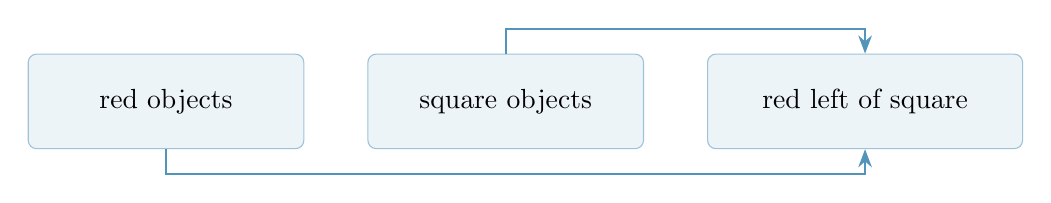
\begin{tikzpicture}[scale=.9]
\node[box,minimum width=35mm] (a) {red objects};
\node[box,minimum width=35mm,right=8mm of a] (b) {square objects};
\node[box,minimum width=40mm,right=8mm of b] (c) {red left of square};
\draw[arrow] (a.south) -- ++(0,-.35) -| (c.south);
\draw[arrow] (b.north) -- ++(0,.35) -| (c.north);
\end{tikzpicture}\end{center}
\vspace{1mm}
\normalsize Can models combine separate concepts like red objects and squares into new spatial arrangements without explicit joint training examples?
\end{frame}

\begin{frame}{Why should anyone care?}
\begin{columns}[T]
\column{.52\textwidth}
\large A model may recognize red items and blue squares separately, yet fail when asked to generate their spatial arrangement.
\vspace{3mm}\\
\normalsize Understanding this failure helps us design more efficient training sets and diagnose compositional generalization limits.
\column{.45\textwidth}
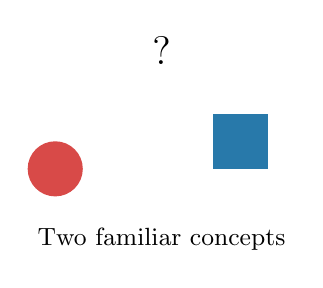
\begin{tikzpicture}
\fill[red] (0,1) circle (.35);\fill[blue] (2,1) rectangle +(0.7,.7);
\node at (1.35,.1) {\small Two familiar concepts};
\node[font=\Large] at (1.35,2.5) {?};
\end{tikzpicture}
\end{columns}
\end{frame}

\begin{frame}{First: what is an image-generation model?}
\begin{center}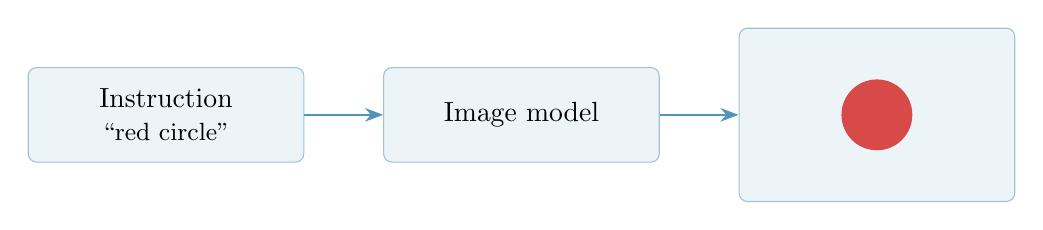
\begin{tikzpicture}[node distance=10mm]
\node[box,minimum width=35mm] (p) {Instruction\\\small ``red circle''};
\node[box,minimum width=35mm,right=of p] (m) {Image model};
\node[box,minimum width=35mm,right=of m,minimum height=22mm] (i) {\tikz\fill[red] (0,0) circle (.45);};
\draw[arrow] (p) -- (m);\draw[arrow] (m) -- (i);
\end{tikzpicture}\end{center}
\vspace{2mm}
\normalsize A conditional model takes an instruction and generates matching pixel arrays, learning visual patterns and statistical dependencies directly from observed training data.
\end{frame}

\begin{frame}{What is an image made of?}
\begin{columns}
\column{.52\textwidth}
\normalsize Digital images are rectangular grids of discrete pixels. Each pixel stores color intensities, so model inputs and outputs are large numeric arrays rather than abstract concepts.
\column{.45\textwidth}\centering
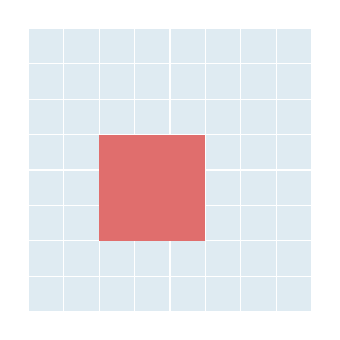
\begin{tikzpicture}[scale=.45]
\foreach \x in {0,...,7} \foreach \y in {0,...,7} {\fill[blue!15] (\x,\y) rectangle +(1,1); \draw[white] (\x,\y) rectangle +(1,1);}
\foreach \x/\y in {2/2,2/3,2/4,3/2,3/3,3/4,4/2,4/3,4/4} \fill[red!80] (\x,\y) rectangle +(1,1);
\end{tikzpicture}
\end{columns}
\end{frame}

\begin{frame}{What is noise?}
\begin{columns}
\column{.5\textwidth}
\normalsize Noise consists of random variations in pixel values. As corruption increases, underlying shapes degrade until the image becomes pure static containing no recognizable visual information.
\column{.5\textwidth}\centering

\begin{tikzpicture}[scale=.32]
\foreach \x in {0,...,11} \foreach \y in {0,...,11} {\pgfmathtruncatemacro{\z}{mod(\x*47+\y*71+\x*\y*23,100)}\fill[black!\z] (\x,\y) rectangle +(1,1);}
\end{tikzpicture}
\end{columns}
\end{frame}

\begin{frame}{Diffusion: learn to reverse noise}
\centering
\begin{tikzpicture}[node distance=9mm]
\node[inner sep=0pt,draw=blue!35] (a) {
\includegraphics[width=25mm]{assets/noise-0.png}};
\node[inner sep=0pt,draw=blue!35,right=of a] (b) {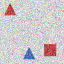
\includegraphics[width=25mm]{assets/noise-1.png}};
\node[inner sep=0pt,draw=blue!35,right=of b] (c) {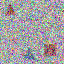
\includegraphics[width=25mm]{assets/noise-2.png}};
\node[inner sep=0pt,draw=blue!35,right=of c] (d) {
\includegraphics[width=25mm]{assets/noise-3.png}};
\draw[arrow] (a) -- (b);\draw[arrow] (b) -- (c);\draw[arrow] (c) -- (d);
\node[below=4mm of b] {\small add noise};
\end{tikzpicture}
\vspace{2mm}\\
\normalsize Forward diffusion progressively corrupts clean images with Gaussian noise. The network learns a prediction that helps reverse the corruption.
\vspace{1mm}\\\captionnote{Illustrative noising, not the model's exact diffusion schedule.}
\end{frame}

\begin{frame}{Generation goes in the other direction}
\centering
\begin{tikzpicture}[node distance=9mm]
\node[inner sep=0pt,draw=blue!35] (a) {
\includegraphics[width=25mm]{assets/noise-3.png}};
\node[inner sep=0pt,draw=blue!35,right=of a] (b) {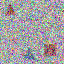
\includegraphics[width=25mm]{assets/noise-2.png}};
\node[inner sep=0pt,draw=blue!35,right=of b] (c) {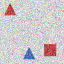
\includegraphics[width=25mm]{assets/noise-1.png}};
\node[inner sep=0pt,draw=blue!35,right=of c] (d) {
\includegraphics[width=25mm]{assets/noise-0.png}};
\draw[arrow] (a)--(b);\draw[arrow] (b)--(c);\draw[arrow] (c)--(d);
\node[below=4mm of b] {\small many denoising steps};
\end{tikzpicture}
\vspace{2mm}\\
\normalsize Generation begins with pure random noise and repeatedly removes predicted noise over many steps, gradually transforming static into a sharp, recognizable visual scene.
\vspace{1mm}\\\captionnote{Conceptual illustration; actual samples are generated by the model.}
\end{frame}

\begin{frame}{Forward diffusion: from image to noise}
\normalsize The forward diffusion process systematically corrupts a clean image $x_0$ across discrete timesteps $t \in \{1, \dots, T\}$ via a Gaussian Markov chain:
\[q(x_t \mid x_{t-1}) = \mathcal{N}\left(x_t;\, \sqrt{1 - \beta_t}\, x_{t-1},\, \beta_t \mathbf{I}\right)\]
\vspace{-2mm}
Using cumulative variance $\bar{\alpha}_t = \prod_{s=1}^t (1 - \beta_s)$, we sample $x_t$ directly in closed form:
\[x_t = \sqrt{\bar{\alpha}_t}\, x_0 + \sqrt{1 - \bar{\alpha}_t}\, \epsilon, \quad \epsilon \sim \mathcal{N}(0, \mathbf{I})\]
\small At timestep $T$, the signal is greatly reduced; the terminal distribution only approximates Gaussian noise.
\end{frame}

\begin{frame}{The reverse process: noise prediction}
\normalsize Generative synthesis reverses corruption by learning parameterized Gaussian transitions:
\[p_\theta(x_{t-1} \mid x_t, c) = \mathcal{N}\left(x_{t-1};\, \mu_\theta(x_t, t, c),\, \sigma_t^2 \mathbf{I}\right)\]
\vspace{-2mm}
Reparameterizing the mean into noise estimation yields the simple MSE objective:
\[\mathcal{L}(\theta) = \mathbb{E}_{t, x_0, \epsilon, c} \left[ \|\epsilon - \epsilon_\theta(x_t, t, c)\|^2 \right]\]
\small This is one common noise-prediction objective. Our later pilot uses velocity prediction.
\end{frame}

\begin{frame}{Backbone architecture: hierarchical U-Net}
\begin{center}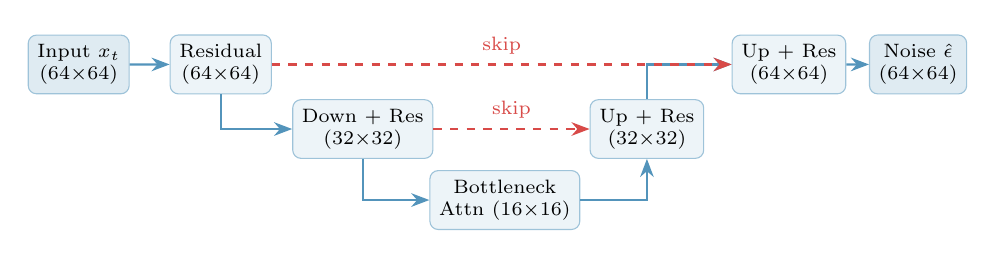
\begin{tikzpicture}[scale=0.82, every node/.style={font=\scriptsize}]
\node[box,minimum height=7mm,fill=blue!15] (in) at (0,2.4) {Input $x_t$\\(64$\times$64)};
\node[box,minimum height=7mm] (e1) at (2.2,2.4) {Residual\\(64$\times$64)};
\node[box,minimum height=7mm] (e2) at (4.4,1.4) {Down + Res\\(32$\times$32)};
\node[box,minimum height=7mm,fill=light] (mid) at (6.6,0.3) {Bottleneck\\Attn (16$\times$16)};
\node[box,minimum height=7mm] (d2) at (8.8,1.4) {Up + Res\\(32$\times$32)};
\node[box,minimum height=7mm] (d1) at (11.0,2.4) {Up + Res\\(64$\times$64)};
\node[box,minimum height=7mm,fill=blue!15] (out) at (13.0,2.4) {Noise $\hat{\epsilon}$\\(64$\times$64)};
\draw[arrow] (in) -- (e1); \draw[arrow] (e1) |- (e2); \draw[arrow] (e2) |- (mid);
\draw[arrow] (mid) -| (d2); \draw[arrow] (d2) |- (d1); \draw[arrow] (d1) -- (out);
\draw[arrow,dashed,red] (e1) -- node[above]{skip} (d1);
\draw[arrow,dashed,red] (e2) -- node[above]{skip} (d2);
\end{tikzpicture}\end{center}
\vspace{1mm}
\normalsize The U-Net combines multi-resolution downsampling and upsampling with skip connections, preserving fine spatial details while capturing global context.
\end{frame}

\begin{frame}{Conditioning via cross-attention}
\begin{center}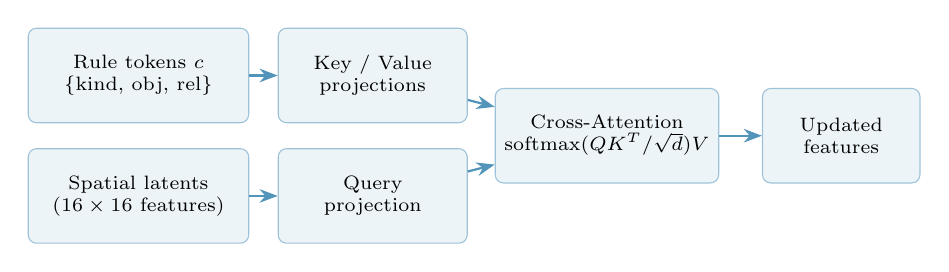
\begin{tikzpicture}[scale=0.85, every node/.style={font=\scriptsize}]
\node[box,minimum width=28mm] (tok) at (0,1.2) {Rule tokens $c$\\$\{\text{kind, obj, rel}\}$};
\node[box,minimum width=24mm] (kv) at (3.5,1.2) {Key / Value\\projections};
\node[box,minimum width=28mm] (feat) at (0,-0.6) {Spatial latents\\($16\times16$ features)};
\node[box,minimum width=24mm] (q) at (3.5,-0.6) {Query\\projection};
\node[box,fill=light,minimum width=26mm] (attn) at (7,0.3) {Cross-Attention\\$\text{softmax}(QK^T/\sqrt{d})V$};
\node[box,minimum width=20mm] (out) at (10.5,0.3) {Updated\\features};
\draw[arrow] (tok) -- (kv); \draw[arrow] (feat) -- (q);
\draw[arrow] (kv) -- (attn); \draw[arrow] (q) -- (attn); \draw[arrow] (attn) -- (out);
\end{tikzpicture}\end{center}
\vspace{1mm}
\normalsize Multi-head cross-attention at the $16\times16$ bottleneck binds symbolic predicate tokens directly to spatial feature maps, guiding object placement and colors.
\end{frame}

\begin{frame}{What does ``conditional'' mean?}
\begin{center}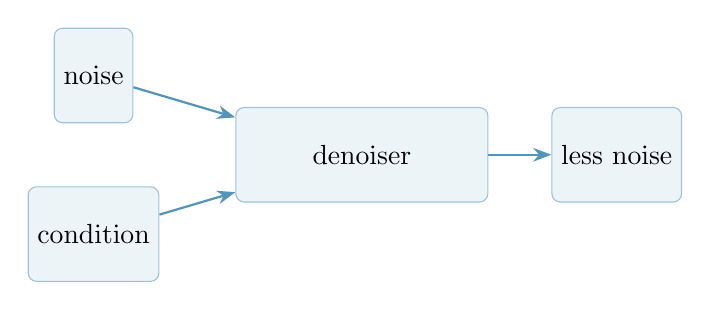
\begin{tikzpicture}[node distance=8mm]
\node[box] (a) {noise};\node[box,below=of a] (b) {condition};
\node[box,minimum width=32mm,right=18mm of $(a)!.5!(b)$] (c) {denoiser};
\node[box,right=of c] (d) {less noise};
\draw[arrow](a)--(c);\draw[arrow](b)--(c);\draw[arrow](c)--(d);
\end{tikzpicture}\end{center}
\vspace{2mm}
\normalsize A conditional diffusion model receives both noisy pixels and an external instruction, guiding each denoising step toward images matching the prompt rather than arbitrary scenes.
\end{frame}

\begin{frame}{Steering generation: classifier-free guidance}
\normalsize Classifier-Free Guidance (CFG) trains conditional and unconditional modes simultaneously by randomly dropping rule tokens ($p_{\text{drop}} = 10\%$) to a learned null embedding $\emptyset$.
\vspace{2mm}\\
During inference, predictions extrapolate along the condition vector:
\[\tilde{\epsilon}_\theta(x_t, c) = \epsilon_\theta(x_t, \emptyset) + s \cdot \left(\epsilon_\theta(x_t, c) - \epsilon_\theta(x_t, \emptyset)\right)\]
\small Setting guidance scale $s > 1$ strengthens adherence to prompt relationships at the expense of sample diversity.
\end{frame}

\begin{frame}{Training and generation are different}
\begin{columns}[T]
\column{.48\textwidth}
\textbf{Training}\\
Clean image + noise\\
$\downarrow$\\
Predict denoising target
\column{.48\textwidth}
\textbf{Generation}\\
Random noise + prompt\\
$\downarrow$\\
Repeated inference
\end{columns}
\vspace{4mm}
\normalsize Training uses known images and controlled noise to teach the denoiser; generation begins with pure noise and relies entirely on prompt guidance.
\end{frame}

\begin{frame}{The scene world we control}
\begin{columns}
\column{.5\textwidth}
\begin{itemize}
\item Synthetic 2D geometric scenes
\item Verifiable bounding boxes and attributes
\item Unambiguous concept exposure counting
\end{itemize}
\column{.46\textwidth}\centering
\includegraphics[width=.72\linewidth]{assets/synthetic-example.png}\\\captionnote{Example generated by the project renderer.}
\end{columns}
\vspace{2mm}
\normalsize We use a controlled synthetic world so concept frequencies and spatial arrangements can be measured with exact mathematical precision.
\end{frame}

\begin{frame}{Our basic visual vocabulary}
\begin{columns}
\column{.48\textwidth}\large\textbf{Colors}\\\textcolor{red}{Red} \quad \textcolor{blue}{Blue}\\\textcolor{green}{Green} \quad Yellow
\column{.48\textwidth}\large\textbf{Shapes}\\Circle \quad Square \\Triangle
\end{columns}
\vspace{4mm}
\normalsize The prototype features four colors and three shapes. Restricting visual primitives isolates core compositional binding mechanisms from natural image complexity.
\vspace{2mm}\\\captionnote{Current prototype vocabulary; the final benchmark is not yet fixed.}
\end{frame}

\begin{frame}{Relationships add structure}
\begin{center}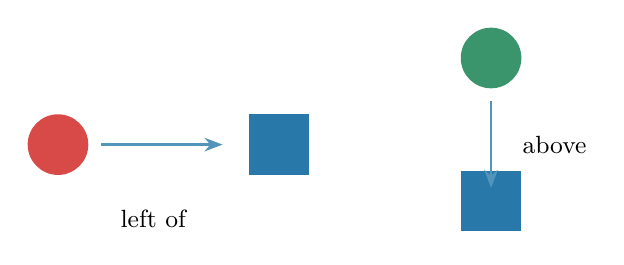
\begin{tikzpicture}[scale=1.1]
\fill[red] (0,0) circle (.35);\fill[blue] (2.2,-.35) rectangle +(0.7,.7);
\draw[arrow] (.5,0) -- (1.9,0);\node[below] at (1.1,-.65) {\small left of};
\fill[green] (5,1) circle (.35);\fill[blue] (4.65,-1) rectangle +(0.7,.7);
\draw[arrow] (5,.5) -- (5,-.5);\node[right] at (5.25,0) {\small above};
\end{tikzpicture}\end{center}
\vspace{1mm}
\normalsize Spatial predicates compare bounding box centers: left requires a smaller horizontal coordinate, while above requires a smaller vertical coordinate across distinct objects.
\end{frame}

\begin{frame}{A rule is a combination of predicates}
\large Example: \textbf{a red object left of a square}.
\vspace{2mm}
\begin{center}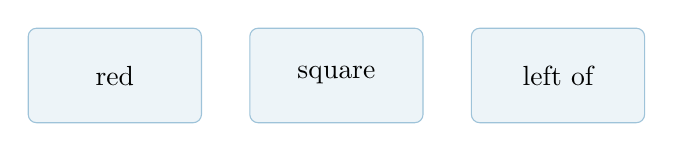
\begin{tikzpicture}[node distance=6mm]
\node[smallbox] (a) {red};\node[smallbox,right=of a] (b) {square};\node[smallbox,right=of b] (c) {left of};
\end{tikzpicture}\end{center}
\vspace{2mm}
\normalsize A composite rule binds multiple predicates together. Each predicate imposes an individual condition (color, shape, or relative position) that must be satisfied simultaneously.
\end{frame}

\begin{frame}{Two roles mean two distinct objects}
\begin{columns}
\column{.5\textwidth}\centering

\begin{tikzpicture}\fill[red] (0,0) circle (.35);\fill[red] (2,-.35) rectangle +(.7,.7);\end{tikzpicture}\\\textbf{Valid:} two red objects
\column{.5\textwidth}\centering

\begin{tikzpicture}\fill[red] (0,0) rectangle +(.7,.7);\end{tikzpicture}\\\textbf{Not enough:} one red square
\end{columns}
\vspace{3mm}
\normalsize Relational rules specify two object roles that must bind to distinct objects. The two objects may share colors, but one object cannot fulfill both roles.
\end{frame}

\begin{frame}{What do we mean by exposure?}
\Large Exposure is how often a pattern appears in the model's training scenes.
\vspace{4mm}\\
\normalsize Exposure is the empirical fraction of training scenes satisfying an event. We compute exposure from verified ground-truth scene annotations, not just prompt requests.
\end{frame}

\begin{frame}{One scene can teach several things}
\begin{columns}
\column{.45\textwidth}\centering
\begin{tikzpicture}\fill[red] (0,0) circle (.4);\fill[blue] (2,-.4) rectangle +(.8,.8);\end{tikzpicture}
\column{.52\textwidth}\begin{itemize}\item A red object appears\item A square appears\item Red is left of a square\end{itemize}
\end{columns}
\vspace{3mm}
\normalsize A single training scene exposes the model to multiple concepts simultaneously: single attributes, pairwise combinations, and complete spatial relationships.
\end{frame}

\begin{frame}{Three levels of exposure}
\begin{center}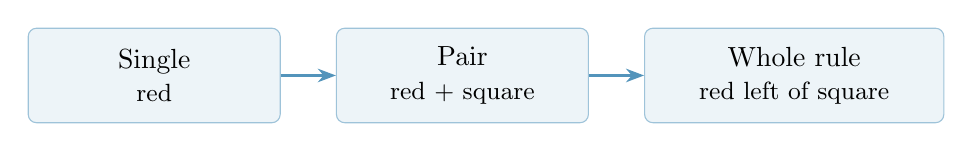
\begin{tikzpicture}[node distance=7mm]
\node[box,minimum width=32mm] (a) {Single\\\small red};
\node[box,minimum width=32mm,right=of a] (b) {Pair\\\small red + square};
\node[box,minimum width=38mm,right=of b] (c) {Whole rule\\\small red left of square};
\draw[arrow](a)--(b);\draw[arrow](b)--(c);
\end{tikzpicture}\end{center}
\vspace{2mm}
\normalsize We evaluate three exposure levels: single features, pairwise co-occurrences, and full rules. Our question is which level best predicts compositional success.
\end{frame}

\begin{frame}{A simple counting example}
\begin{center}
\begin{tikzpicture}
\foreach \i in {0,...,9} {\fill[blue!20] (\i*.65,0) rectangle +(0.5,0.5);}
\foreach \i in {0,...,2} {\fill[red!75] (\i*.65,0) rectangle +(0.5,0.5);}
\node[below] at (3,-.2) {10 training scenes};
\end{tikzpicture}\end{center}
\vspace{1mm}
\normalsize When 3 of 10 sampled scenes satisfy a rule, its empirical exposure is 30\%. In real datasets, finite sampling creates uncertainty that requires statistical estimation.
\end{frame}

\begin{frame}{Why single-concept counts are not enough}
\begin{columns}
\column{.48\textwidth}\centering\textbf{Dataset A}\\\vspace{1mm}
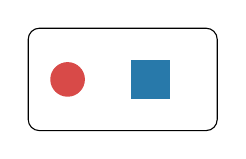
\begin{tikzpicture}\draw[rounded corners] (-.3,-.3) rectangle (2.1,1);\fill[red] (.2,.35) circle (.22);\fill[blue] (1,.1) rectangle +(0.5,0.5);\end{tikzpicture}\\Concepts appear together.
\column{.48\textwidth}\centering\textbf{Dataset B}\\\vspace{1mm}
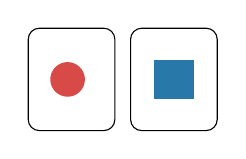
\begin{tikzpicture}\draw[rounded corners] (-.3,-.3) rectangle (.8,1);\draw[rounded corners] (1,-.3) rectangle (2.1,1);\fill[red] (.2,.35) circle (.22);\fill[blue] (1.3,.1) rectangle +(.5,.5);\end{tikzpicture}\\Concepts appear separately.
\end{columns}
\vspace{3mm}
\normalsize Both datasets can share identical individual concept frequencies, yet differ completely in joint co-occurrence. Marginal counts alone hide these joint exposure differences.
\end{frame}

\begin{frame}{Lift: is a combination common or rare?}
\normalsize Lift compares observed joint exposure against an independent product reference:
\[\text{lift} = \log\!\left(\frac{\text{observed combination exposure}}{\text{product of individual exposures}}\right)\]
\begin{itemize}
\item Positive lift: concepts co-occur more often than expected by chance
\item Negative lift: concepts co-occur less often than expected
\end{itemize}
\captionnote{The product baseline is a reference; shared objects induce dependencies.}
\end{frame}

\begin{frame}{Illustrating lift with numbers}
\begin{center}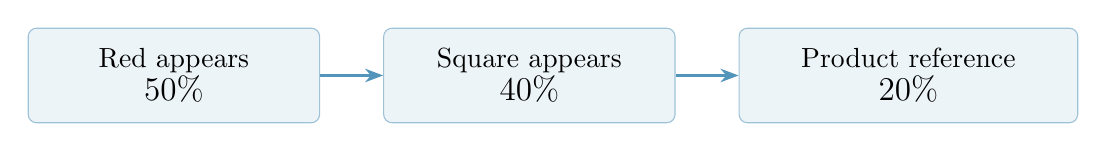
\begin{tikzpicture}
\node[box,minimum width=37mm] (a) {Red appears\\\large 50\%};
\node[box,minimum width=37mm,right=8mm of a] (b) {Square appears\\\large 40\%};
\node[box,minimum width=43mm,right=8mm of b] (c) {Product reference\\\large 20\%};
\draw[arrow](a)--(b);\draw[arrow](b)--(c);
\end{tikzpicture}\end{center}
\vspace{2mm}
\normalsize If red appears in 50\% of scenes and square in 40\%, independence predicts a 20\% baseline. An observed 10\% joint rate yields negative lift.
\end{frame}

\begin{frame}{How do we measure model success?}
\begin{center}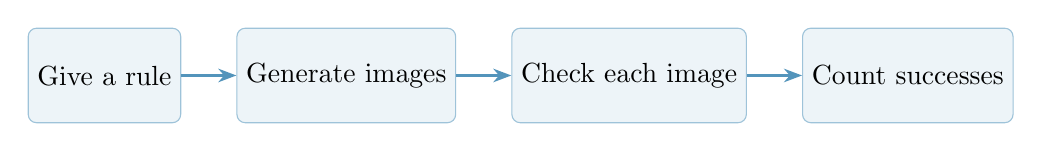
\begin{tikzpicture}[node distance=7mm]
\node[box] (a) {Give a rule};\node[box,right=of a] (b) {Generate images};
\node[box,right=of b] (c) {Check each image};\node[box,right=of c] (d) {Count successes};
\draw[arrow](a)--(b);\draw[arrow](b)--(c);\draw[arrow](c)--(d);
\end{tikzpicture}\end{center}
\[\text{Observed success} = \frac{\text{classified images satisfying the rule}}{\text{total classified images}}\]
\vspace{1mm}
\normalsize We evaluate generated images with an automated checker, reporting success rates while tracking and reporting checker abstentions separately from model generation errors.
\end{frame}

\begin{frame}{A reference for composition}
\normalsize If constituent abilities combine independently, expected joint success equals the product of individual accuracies (for instance, $0.8 \times 0.7 = 0.56$).
\vspace{3mm}\\
\normalsize Because shared objects induce dependencies, this calculation provides a testable empirical reference rather than an absolute theoretical performance ceiling.
\end{frame}

\begin{frame}{The composition gap}
\begin{center}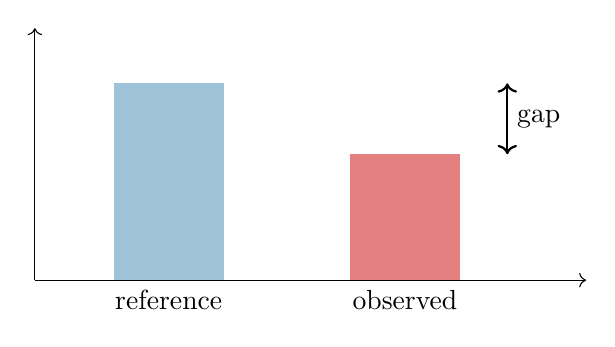
\begin{tikzpicture}
\draw[->] (0,0)--(0,3.2);\draw[->] (0,0)--(7,0);
\fill[blue!45] (1,0) rectangle (2.4,2.5);\fill[red!70] (4,0) rectangle (5.4,1.6);
\node[below] at (1.7,0) {reference};\node[below] at (4.7,0) {observed};
\draw[<->,thick] (6,1.6)--(6,2.5);\node[right] at (6,2.05) {gap};
\end{tikzpicture}\end{center}
\vspace{1mm}
\normalsize The composition gap measures the deficit between observed rule success and the product reference, quantifying the extra difficulty of binding concepts together.
\vspace{1mm}\\\captionnote{Illustration only; bars do not represent measured project results.}
\end{frame}

\begin{frame}{What does a zero gap mean?}
\large When observed success equals the product reference, the gap is \textbf{zero}.
\vspace{3mm}\\
\normalsize A zero gap means observed success equals the chosen product reference. The proposal uses logit scale; working drafts also explore a log-scale version.
\end{frame}

\begin{frame}{Our main hypotheses}
\begin{itemize}
\item \textbf{Complexity scaling:} Multi-predicate rules suffer larger negative composition gaps.
\item \textbf{Joint exposure benefit:} Higher joint training exposure directly improves rule success.
\item \textbf{Pairwise transfer:} Seeing pairs helps models generalize to unseen full combinations.
\end{itemize}
\vspace{2mm}
\small These hypotheses define the core empirical questions our study tests.
\end{frame}

\begin{frame}{A separate question: how much is enough?}
\Large \textbf{N50}: an exposure level associated with 50\% success.
\vspace{4mm}\\
\normalsize Rather than evaluating a single arbitrary training checkpoint, we trace exposure-response curves. N50 marks where accuracy crosses 50\%, measuring sample efficiency for rule learning.
\end{frame}

\begin{frame}{An illustrative learning curve}
\centering\begin{tikzpicture}[scale=.85]
\draw[->] (0,0)--(9,0) node[right]{exposure};\draw[->] (0,0)--(0,3.6) node[above]{success};
\draw[dashed] (0,1.8)--(8,1.8);\node[left] at (0,1.8) {50\%};
\draw[blue,very thick] plot[smooth] coordinates {(0.4,.25) (2,.5) (4,1.7) (6,2.8) (8,3.1)};
\draw[dashed,red] (4.2,0)--(4.2,1.8);\node[below] at (4.2,0) {N50};
\end{tikzpicture}\\
\vspace{1mm}
\normalsize Conceptual learning curves illustrate the transition toward mastery. Estimating N50 requires training allocations that span above and below the threshold without unsafe extrapolation.
\vspace{1mm}\\\captionnote{Illustration only; not a fitted result.}
\end{frame}

\begin{frame}{Model optimization: AdamW and EMA}
\normalsize Weights are optimized by minimizing mean squared error with \textbf{AdamW}:
\[\theta_{k+1} = \theta_k - \eta_k \, \frac{\hat{m}_k}{\sqrt{\hat{v}_k} + \epsilon_{\text{opt}}} - \lambda \eta_k \theta_k\]
\vspace{-2mm}
To smooth parameter updates, an \textbf{Exponential Moving Average (EMA)} shadow model is maintained:
\[\theta_{\text{EMA}} \leftarrow \mu \, \theta_{\text{EMA}} + (1 - \mu) \, \theta_k \quad (\mu = 0.999)\]
\small The pilot sampler uses EMA weights; better perceptual quality is not guaranteed.
\end{frame}

\begin{frame}{Inference optimization: sampling schedules}
\begin{columns}[T]
\column{.48\textwidth}
\textbf{DDPM (Stochastic Markovian)}\\
\begin{itemize}
\item Ancestral reverse sampling
\item Injects Gaussian noise at each step
\item Requires 100--1000 sequential passes
\end{itemize}
\column{.48\textwidth}
\textbf{DDIM (Deterministic Non-Markov)}\\
\begin{itemize}
\item Continuous ODE trajectory
\item Deterministic mapping from noise
\item Accelerates inference to 20--50 steps
\end{itemize}
\end{columns}
\vspace{4mm}
\normalsize DDIM and higher-order ODE solvers dramatically accelerate inference throughput without sacrificing visual fidelity or rule satisfaction.
\end{frame}

\begin{frame}{How do we change exposure fairly?}
\begin{center}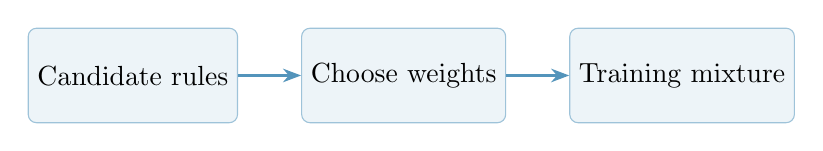
\begin{tikzpicture}[node distance=8mm]
\node[box] (a) {Candidate rules};\node[box,right=of a] (b) {Choose weights};
\node[box,right=of b] (c) {Training mixture};\draw[arrow](a)--(b);\draw[arrow](b)--(c);
\end{tikzpicture}\end{center}
\vspace{2mm}
\normalsize To isolate joint exposure, we adjust training mixture probabilities. This shifts how often whole rules appear while holding individual concept frequencies closely matched across datasets.
\end{frame}

\begin{frame}{The exposure matrix}
\begin{columns}
\column{.53\textwidth}
\normalsize The exposure matrix maps requested conditions (columns) to realized visual events (rows). Cell entries are estimated by sampling ground-truth annotations rather than guessing from prompt labels alone.
\column{.43\textwidth}\centering

\begin{tikzpicture}[scale=.55]
\foreach \x in {0,...,3} \foreach \y in {0,...,3} {\pgfmathtruncatemacro{\v}{20+mod(\x*31+\y*23,65)}\fill[blue!\v] (\x,\y) rectangle +(1,1);\draw[white] (\x,\y) rectangle +(1,1);}
\end{tikzpicture}
\end{columns}
\vspace{2mm}\captionnote{Illustrative matrix; actual values estimated from sampled annotations.}
\end{frame}

\begin{frame}{Exposure design as constrained optimization}
\normalsize Finding balanced training mixtures is framed as convex optimization over condition weights $w \in \Delta^{K-1}$:
\[\min_{w} \; D_{\text{KL}}(w \,\|\, u) = \sum_{k=1}^K w_k \log(K w_k)\]
\vspace{-2mm}
subject to equality and inequality exposure constraints:
\[\mathbf{M}_{\text{marginal}} w = b_{\text{matched}}, \quad l \le \mathbf{M}_{\text{joint}} w \le u, \quad \sum w_k = 1, \; w_k \ge 0\]
\small Solving this via SLSQP produces the maximally uniform mixture that cleanly separates joint exposure.
\end{frame}

\begin{frame}{A controlled comparison}
\begin{columns}[T]
\column{.48\textwidth}\textbf{Mixture A}\begin{itemize}\item Concepts matched\item Lower joint exposure\end{itemize}
\column{.48\textwidth}\textbf{Mixture B}\begin{itemize}\item Concepts matched\item Higher joint exposure\end{itemize}
\end{columns}
\vspace{4mm}
\normalsize Comparing models trained on Mixtures A and B reveals whether joint co-occurrence drives compositional learning when individual concept frequencies remain strictly matched.
\end{frame}

\begin{frame}{Why do we need a checker?}
\begin{center}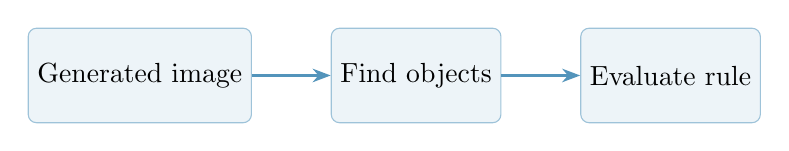
\begin{tikzpicture}[node distance=10mm]
\node[box] (a) {Generated image};\node[box,right=of a] (b) {Find objects};
\node[box,right=of b] (c) {Evaluate rule};\draw[arrow](a)--(b);\draw[arrow](b)--(c);
\end{tikzpicture}\end{center}
\vspace{2mm}
\normalsize An automated checker detects objects and tests spatial relations from pixels. This provides repeatable, standardized evaluation across thousands of generated images without subjective human grading.
\end{frame}

\begin{frame}{The checker can also be wrong}
\begin{columns}[T]
\column{.48\textwidth}\textbf{False accept}\\Checker says yes, but the image violates the rule.
\column{.48\textwidth}\textbf{False reject}\\Checker says no, but the image satisfies the rule.
\end{columns}
\vspace{4mm}
\normalsize When ambiguity prevents classification, the checker records an \textbf{abstention}. Abstentions must be tracked separately rather than treated as generation failures.
\end{frame}

\begin{frame}{Humans help validate the checker}
\begin{center}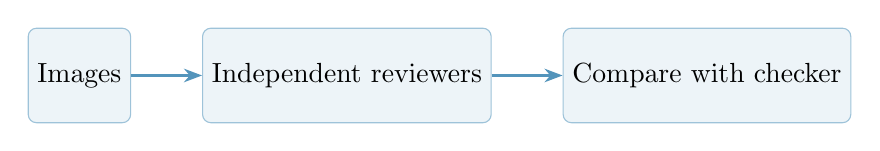
\begin{tikzpicture}[node distance=9mm]
\node[box] (a) {Images};\node[box,right=of a] (b) {Independent reviewers};
\node[box,right=of b] (c) {Compare with checker};\draw[arrow](a)--(b);\draw[arrow](b)--(c);
\end{tikzpicture}\end{center}
\vspace{2mm}
\normalsize Before trusting the checker, human reviewers audit at least 300 complexity-stratified images. Comparing verdicts against the checker measures false accepts, false rejects, and per-predicate errors.
\end{frame}

\begin{frame}{Why blind the review?}
\begin{columns}[T]
\column{.52\textwidth}
\normalsize Reviewers inspect synthesized images alongside target questions without seeing automated checker predictions or training labels.
\vspace{3mm}\\
\normalsize Blinding reduces the risk that checker predictions influence human judgments; it does not guarantee reviewer independence or perfect labels.
\column{.44\textwidth}
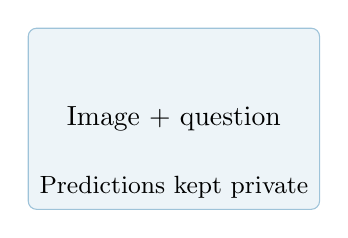
\begin{tikzpicture}\node[box,minimum width=37mm,minimum height=23mm] {Image + question};\node[below=6mm,align=center] {\small Predictions kept private};\end{tikzpicture}
\end{columns}
\end{frame}

\begin{frame}{What does the current model produce?}
\begin{columns}
\column{.48\textwidth}\centering
\includegraphics[width=.72\linewidth]{assets/pilot-red.png}\\\small Requested: red
\column{.48\textwidth}\centering
\includegraphics[width=.72\linewidth]{assets/pilot-relation.png}\\\small Requested: blue above circle
\end{columns}
\vspace{2mm}
\normalsize Exploratory samples from the 800,000-update pilot show basic color generation, but multi-object relations show artifacts. These illustrate current prototypes rather than measured benchmark accuracy.
\end{frame}

\begin{frame}{What have we built?}
\begin{itemize}
\item Synthetic scene renderer and symbolic rule evaluator
\item Exposure measurement and mixture optimization tools
\item Pilot diffusion checkpoints, checkers, and review interfaces
\end{itemize}
\vspace{3mm}
\normalsize Software components are operational, but completing infrastructure is distinct from validating the benchmark or running the full experiment.
\end{frame}

\begin{frame}{What has the team reviewed?}
\begin{itemize}
\item Conducted blinded calibration trials on small sample sets
\item Discussed edge-case disagreements to refine rubrics
\item Recorded and reported checker abstentions transparently
\end{itemize}
\vspace{2mm}
\normalsize A 300-image, four-condition pilot audit pack is prepared; however, full complexity-stratified benchmark coverage remains outstanding.
\end{frame}

\begin{frame}{One current obstacle: checker coverage}
\Large Some recognizable images are rejected by strict pixel and geometry checks.
\vspace{4mm}\\
\normalsize The prototype checker enforces strict color and geometric heuristics, causing false rejections. More flexible thresholds improve recall but require independent validation against false accepts.
\end{frame}

\begin{frame}{One current obstacle: relation exposure}
\Large An unrestricted relation can be almost always true in a three-object scene.
\vspace{4mm}\\
\normalsize When spatial relations are tested without attribute constraints, multiple objects make relations like 'left of' almost trivially true. Full attributed rules represent completely different events.
\end{frame}

\begin{frame}{One current obstacle: experimental design}
\Large We need designs that vary combinations while keeping other exposures controlled.
\vspace{4mm}\\
\normalsize Current exploratory allocations fail the proposal's decorrelation targets and variance inflation criteria. Refined mathematical optimization is required to prevent confounding concept drift.
\end{frame}

\begin{frame}{Stage 0: checks before the main study}
\begin{itemize}
\item Human audit validation of automated checkers
\item Exposure decorrelation and design stability
\item Baseline comparison against adapted MOSAIC protocols
\end{itemize}
\vspace{3mm}
\normalsize \textbf{Current status: not passed.} Main experimental model training will proceed only after all three Stage 0 validation gates are met.
\end{frame}

\begin{frame}{What happens after the gates?}
\begin{center}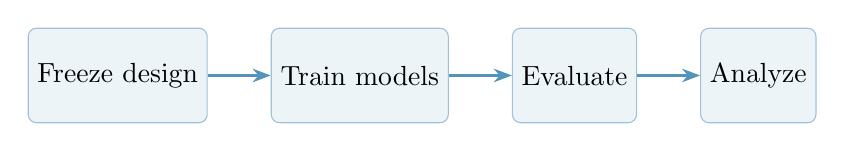
\begin{tikzpicture}[node distance=8mm]
\node[box] (a) {Freeze design};\node[box,right=of a] (b) {Train models};
\node[box,right=of b] (c) {Evaluate};\node[box,right=of c] (d) {Analyze};
\draw[arrow](a)--(b);\draw[arrow](b)--(c);\draw[arrow](c)--(d);
\end{tikzpicture}\end{center}
\vspace{2mm}
\normalsize Once validation gates pass, we will freeze benchmark specifications, train controlled diffusion models, evaluate generated images with checkers, and analyze resulting composition gaps.
\vspace{1mm}\\\captionnote{Planned workflow, not completed research findings.}
\end{frame}

\begin{frame}{Possible outcome: joint exposure matters}
\large Heightened joint exposure could significantly improve multi-concept generation, even when individual concept frequencies are perfectly matched.
\vspace{4mm}\\
\normalsize This positive finding would demonstrate that compositional binding requires dedicated co-occurrence examples during training, guiding future dataset construction.
\end{frame}

\begin{frame}{Possible outcome: the hypothesis fails}
\large Increased joint exposure might yield minimal benefit, or effects could vary across rule types.
\vspace{4mm}\\
\normalsize A negative result would be equally informative, suggesting that generative models generalize spatial arrangements compositionally from constituent exposure without needing explicit joint pairings.
\end{frame}

\begin{frame}{Real-world implications: medical imaging}
\begin{columns}[T]
\column{.55\textwidth}
\begin{itemize}
\item \textbf{Rare co-morbidities:} Clinical scans frequently show individual pathologies, but dual conditions (e.g., effusion + cardiomegaly) are exceptionally sparse.
\item \textbf{Diagnostic safety:} Synthetic augmentation requires verified attribute binding to avoid hallucinating false organ-lesion couplings.
\item \textbf{Exposure thresholds:} Measuring $N_{50}$ isolates the minimal co-occurrence needed for clinically faithful scan synthesis.
\end{itemize}
\column{.43\textwidth}\centering
\vspace{1mm}
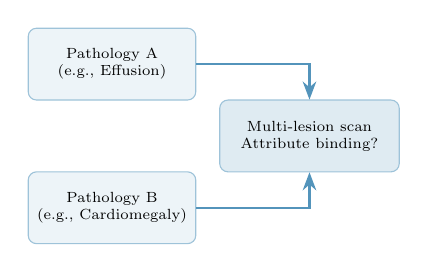
\begin{tikzpicture}[scale=0.76, every node/.style={transform shape, font=\scriptsize}]
\node[box,minimum width=28mm,fill=light] (a) at (0,1.2) {Pathology A\\(e.g., Effusion)};
\node[box,minimum width=28mm,fill=light] (b) at (0,-1.2) {Pathology B\\(e.g., Cardiomegaly)};
\node[box,minimum width=30mm,fill=blue!15] (c) at (3.3,0) {Multi-lesion scan\\Attribute binding?};
\draw[arrow] (a.east) -| (c.north);
\draw[arrow] (b.east) -| (c.south);
\end{tikzpicture}
\end{columns}
\vspace{3mm}
\captionnote{Controlled exposure reveals whether clinical models generalize to rare joint diseases.}
\end{frame}

\begin{frame}{Real-world implications: robotics and safety}
\begin{itemize}
\item \textbf{Autonomous vehicles:} Rare safety-critical corner cases combine familiar entities in unseen configurations (e.g., pedestrian behind an open vehicle door in fog).
\item \textbf{Robotic manipulation:} Goal-image generation for robot policies demands strict geometric binding between grasp targets and surrounding obstacles.
\item \textbf{Defect simulation:} Industrial inspection models must simulate multi-defect interactions from sparse marginal failure observations.
\end{itemize}
\vspace{2mm}
\normalsize Our exposure-control framework provides the mathematical foundation to audit whether generative simulators reliably synthesize hazardous edge cases.
\end{frame}

\begin{frame}{Why this research matters}
\begin{itemize}
\item Clarifies whether generative models require joint observations
\item Establishes rigorous methods to measure realized training exposure
\item Guides principled allocation of compute and dataset collection budgets
\end{itemize}
\vspace{2mm}
\normalsize Empirical measurement replaces guesswork in training set design for compositional image generation.
\end{frame}

\begin{frame}{Take-home message}
\Large A model's success may depend on \textbf{which combinations} it has seen, not only how often it has seen the pieces.
\vspace{4mm}\\
\normalsize By controlling synthetic environments, tracking true exposures, and auditing checkers, our project tests whether joint training examples drive compositional skill.
\end{frame}

\begin{frame}{Questions?}
\centering{\Huge Thank you}
\vspace{6mm}\\
\normalsize
\textbf{Core question:} Which training examples help a model combine concepts?
\vspace{3mm}\\
{\small Open for questions regarding synthetic controls, exposure metrics, checker validation, and next experimental steps.}
\end{frame}

\begin{frame}{References and project evidence}
\small
\begin{itemize}
\item \emph{Which Exposure Matters?} Research proposal, revision 4.
\item Jeong et al., MOSAIC, ICML 2026: controlled scene complexity and imbalance.
\item Okawa et al., NeurIPS 2023: compositional abilities and constituent abilities.
\item Nützel et al., GRASP, arXiv 2025: gradient conflicts in long-tail diffusion.
\item Bradley, ICML 2026: local conditional scores in compositional diffusion.
\item Project documentation: stage status, checker, human audit and exposure design.
\end{itemize}
\vspace{2mm}\captionnote{Prior-work descriptions follow the proposal; consult the original publications for details.}
\end{frame}
\end{document}
